\documentclass[11pt]{article}
\usepackage{fullpage}
\usepackage{amsmath,amsthm,amssymb,amsfonts,multirow}
\usepackage{mathtools}
\usepackage{graphicx}
\usepackage{xcolor}
\usepackage{float}
%\usepackage{enumerate}
\usepackage[shortlabels, inline]{enumitem}
\usepackage{textcomp}
\usepackage{hyperref}
\usepackage{comment}

\usepackage{listings}
\lstset{language=Python, numbers=left, basicstyle=\ttfamily, keywordstyle=\color{blue}, showstringspaces=false}

\usepackage[style=alphabetic-verb]{biblatex}
% \bibliography{Problems/ref.bib}

\newcommand{\N}{\mathbb{N}}
\newcommand{\Z}{\mathbb{Z}}
\newcommand{\Q}{\mathbb{Q}}
\newcommand{\R}{\mathbb{R}}
\newcommand{\C}{\mathcal{C}}
\newcommand{\K}{\mathbb{K}}
\renewcommand{\div}{\mid}
\newcommand{\ndiv}{\nmid}
\newcommand{\E}{\mathbb{E}}
\newcommand{\I}{\mathbb{I}}
\newcommand{\F}{\mathcal{F}}

\DeclareMathOperator{\id}{Id}
\DeclareMathOperator{\tr}{Tr}
\DeclareMathOperator*{\argmax}{arg\,max}
\DeclareMathOperator*{\argmin}{arg\,min}
\DeclareMathOperator{\lcm}{lcm}
\DeclareMathOperator{\spn}{span}
\DeclareMathOperator{\acosh}{acosh}

\DeclarePairedDelimiter{\floor}{\lfloor}{\rfloor}
\DeclarePairedDelimiter{\ceil}{\lceil}{\rceil}
\DeclarePairedDelimiter{\abs}{\lvert}{\rvert}

\newcommand{\subtag}[1]{\tag{\theparentequation#1}}

\renewcommand{\vec}[1]{\mathbf{#1}}

\usepackage{subfiles}
\usepackage{subcaption}
\makeatletter
\newcommand\nocaption{
    \renewcommand\p@subfigure{}
    \renewcommand{\thesubfigure}{\arabic{figure}\alph{subfigure}}
}
\makeatother


\newenvironment{problem}[2][Question]{\begin{trivlist}
\item[\hskip \labelsep {\bfseries #1}\hskip \labelsep {\bfseries #2.}]}{\end{trivlist}}

\newenvironment{solution}{%
  \begin{proof}[\textbf{Solution}]$ $\par\nobreak\ignorespaces
}{%
  \end{proof}
}

\theoremstyle{definition}
\newtheorem{definition}{Definition}
\newtheorem{theorem}{Theorem}
\newtheorem{lemma}{Lemma}

\hypersetup{
    colorlinks=true,
    linkcolor=blue,
    filecolor=magenta,      
    urlcolor=cyan,
    pdftitle={Overleaf Example},
    pdfpagemode=FullScreen,
    }


\title{Intro to Computational Mathematics: Section 10}
\date{November 2025}

\begin{document}
\maketitle

\begin{problem}{5.6.1}
For each integral below, use \href{https://fncbook.com/integration/#function-trapezoid}{Function 5.6.1} to estimate the integral for $n = 10 \cdot 2^k$ nodes for $k = 1, 2, \ldots, 10$. Make a log-log plot of the errors and confirm or refute second-order accuracy. (These integrals were taken from \href{https://doi.org/10.1080/10586458.2005.10128931}{Bailey \textit{et al.} (2005)}.)
\begin{enumerate}[(a)]
    \item $\int_0^1 x\log(1 + x)\, dx = \frac{1}{4}$
    \item $\int_0^1 x^2 \tan^{-1}x \, dx = \frac{\pi - 2 + 2\log 2}{12}$
    \item $\int_0^{\pi/2} e^x \cos x \, dx = \frac{e^{\pi/2} - 1}{2}$
    \item $\int_0^1 \sqrt{x}\log(x) \, dx = - \frac{4}{9}$ (Note: Although the integrand has the limiting value zero as $x \rightarrow 0$, it cannot be evaluated naively at $x = 0$. You can start the integral at $\epsilon_{\text{mach}}$ instead.)
    \item $\int_0^1 \sqrt{1 - x^2} \, dx = \frac{\pi}{4}$
\end{enumerate}
\end{problem}
\begin{solution}
The following code compute the trapezoid rule quadrature for each the given functions:
\begin{lstlisting}
import numpy as np
import matplotlib.pyplot as plt

def trapezoid(f, a, b, n):
    """
    trapezoid(f, a, b, n)

    Apply the trapezoid integration formula for integrand f over interval [a,b], broken up into n equal pieces. Returns estimate, vector of nodes, and vector of integrand values at the nodes.
    """
    h = (b - a) / n
    t = np.linspace(a, b, n + 1)
    y = f(t)
    T = h * (np.sum(y[1:-1]) + 0.5 * (y[0] + y[-1]))
    return T, t, y

def f_a(x):
    return x * np.log(1 + x)

def f_b(x):
    return x**2 * np.atan(x)

def f_c(x):
    return np.exp(x) * np.cos(x)

def f_d(x):
    return np.sqrt(x) * np.log(x)

def f_e(x):
    return np.sqrt(1 - x**2)

def plot_errors(f, soln, a, b, label):
    n = [10 * 2**(i + 1) for i in range(10)]
    err = []
    for n_ in n:
        T, _, _ = trapezoid(f, a, b, n_)
        err.append(abs(soln - T))
    plt.plot(np.log(n), np.log(err), label=label)

plot_errors(f_a, 1/4, 0, 1, 'a')
plot_errors(f_b, (np.pi - 2 + 2*np.log(2))/12, 0, 1, 'b')
plot_errors(f_c, (np.exp(np.pi/2) - 1)/2, 0, np.pi/2, 'c')
plot_errors(f_d, -4/9, np.finfo(float).eps, 1, 'd')
plot_errors(f_e, np.pi/4, 0, 1, 'e')
plt.xlabel('log(n)')
plt.ylabel('log(err)')
plt.title('Convergence of Trapezoid Rule Quadrature')
plt.legend()
plt.show()
\end{lstlisting}
Output:
\begin{center}
    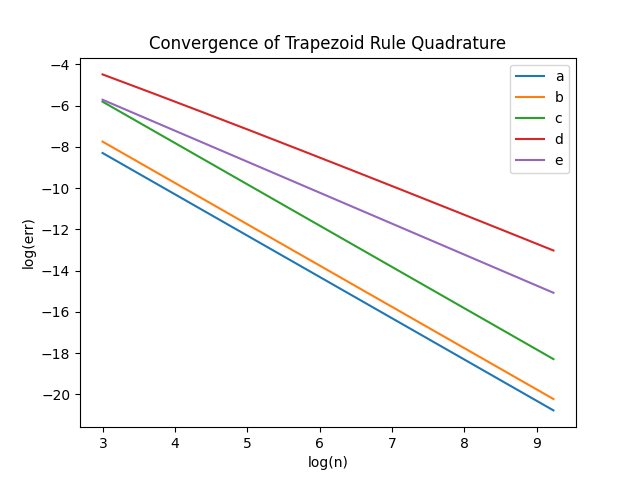
\includegraphics[width=0.8\textwidth]{5.6.1_fig.png}
\end{center}
\end{solution}




\begin{problem}{5.6.8}
For the integrals in (a)-(c) of \href{https://fncbook.com/integration/#problem-integration-tests}{Exercise 5.6.1}, extrapolate the trapezoidal results for $n = 32, 48, 72, 108, 162$ two levels to get sixth-order accurate results, and make a table of the errors.
\end{problem}
\begin{solution}
The following code compute the extrapolation of the trapezoid rule quadrature for each the given functions:
\begin{lstlisting}
import numpy as np
import matplotlib.pyplot as plt

def extrapolate_6th_order(f, a, b, n):
    """
    extrapolate_6th_order(f, a, b, n)

    Apply the trapezoid integration formula followed by two steps of extrapolation
     for integrand f over interval [a,b], broken up into n equal pieces.
     Returns 6th order estimate.
    """
    h = (b - a) / n
    t = np.linspace(a, b, n + 1)
    y = f(t)
    T = np.zeros(3)

    T[0] = h * (np.sum(y[1:-1]) + 0.5 * (y[0] + y[-1]))

    # 2nd order
    n = 2 * n
    h = h / 2
    t = h * np.arange(n + 1)
    T[1] = T[0] / 2 + h * sum(f(t[1:-1:2]))

    # 4th order
    n = 2 * n
    h = h / 2
    t = h * np.arange(n + 1)
    T[2] = T[1] / 2 + h * sum(f(t[1:-1:2]))

    S = np.array([(4 * T[i + 1] - T[i]) / 3 for i in range(2)])

    # 6th order
    R = (16 * S[1] - S[0]) / 15
    return R

def f_a(x):
    return x * np.log(1 + x)

def f_b(x):
    return x**2 * np.atan(x)

def f_c(x):
    return np.exp(x) * np.cos(x)

def extrapolate(f, soln, a, b):
    n = [32, 48, 72, 108, 162]
    err = []
    for n_ in n:
        est = extrapolate_6th_order(f, a, b, n_)
        err.append(abs(soln - est))
    return err

print('n = ' + str([32, 48, 72, 108, 162]))
print('a: ' + str(extrapolate(f_a, 1/4, 0, 1)))
print('b: ' + str(extrapolate(f_b, (np.pi - 2 + 2*np.log(2))/12, 0, 1)))
print('c: ' + str(extrapolate(f_c, (np.exp(np.pi/2) - 1)/2, 0, np.pi/2)))
\end{lstlisting}
Output:

\begin{tabular}{c|c|c|c}
    n \textbackslash \,f & $f_a$ & $f_b$ & $f_c$ \\\hline
    32 & 1.3877787807814457e-14 & 2.2593038551121936e-14 & 1.6830981053317373e-13 \\
    48 & 1.2212453270876722e-15 & 1.915134717478395e-15 & 1.509903313490213e-14 \\
    72 & 2.7755575615628914e-17 & 1.1102230246251565e-16 & 2.4424906541753444e-15 \\
    108 & 1.3877787807814457e-16 & 2.7755575615628914e-17 & 4.440892098500626e-16 \\
    162 & 5.551115123125783e-17 & 0.0 & 4.440892098500626e-16
\end{tabular}
\end{solution}



\begin{problem}{Q2}
As seen on the midterm \texttt{(i.e., Section \#2)}, consider
$$ 
f(x) = \log(\exp(x) + \exp(-x)) \ .  $$
Evaluating this function directly can be unstable. This time, let's evaluate its derivatives.\\
\begin{enumerate}[(a)]
\item The derivative of $f$ is given by $f'(x) = \frac{\exp(x) - \exp(-x)}{\exp(x) + \exp(-x)}$. \\
Is $f'$ reasonably well-conditioned at $x = 1.23$? \\
\item Consider numerically approximating $f'(1.23)$ for a given stepsize $h>0$ via the formula 
$$ \frac{f(1.23 + h) - f(1.23)}{h} .$$
If implemented in standard floating point arithmetic, what value of $h$ would you recommend using to minimize the difference from the true answer $f'(1.23)$?
\item  What values of $a,b,c\in\mathbb{R}$ maximize the order of accuracy for approximating $f'(0)$ below? 
$$ \frac{a f(-h) + bf(0) + cf(2h)}{h} $$
\end{enumerate}
\end{problem}
\begin{solution}
\begin{enumerate}[(a)]
\item
\begin{align*}
    \kappa_{f'}(x) &= \abs*{\frac{x(f')'(x)}{(f')(x)}} \\
    &= \abs*{\frac{x f''(x)}{f'(x)}} \\
    &= \abs*{x \frac{(e^x + e^{-x})^2 - (e^x - e^{-x})^2}{(e^x + e^{-x})^2} \frac{e^x + e^{-x}}{e^{x} - e^{-x}}} \\
    &= \abs*{x \frac{e^{2x} + 2e^x e^{-x} + e^{-2x} - e^{2x} + 2e^x e^{-x} - e^{-2x}}{(e^x + e^{-x})^2} \frac{e^x + e^{-x}}{e^{x} - e^{-x}}} \\
    &= \abs*{x \frac{4}{(e^x + e^{-x})^2} \frac{e^x + e^{-x}}{e^{x} - e^{-x}}} \\
    &= \abs*{\frac{4x}{e^{2x} - e^{-2x}}} \\
    \kappa_{f'}(1.23) &= \abs*{\frac{4(1.23)}{e^{2(1.23)} - e^{-2(1.23)}}} \\
    &\approx 4/9
\end{align*}
So computing $f'$ this way is reasonably well conditioned at $x = 1.23$.
\item
Using the Taylor approximation of $f(x)$, we have that $f'(1.23) - \frac{f(1.23 + h) - f(1.23)}{h} = f'(1.23) - \frac{[f(1.23) + hf'(1.23) + \frac{h^2}{2}f''(1.23) + O(h^3)] - f(1.23)}{h} = \frac{h}{2}f''(1.23) + O(h^2)$.

Thus this approach has accuracy of order $1$ which trades off with the order $O(\epsilon_{\text{mach}}/h)$ accuracy from the subtractive cancellation in computing $f(1.23 + h) - f(1.23)$.

We therefore want to minimize the error by minimizing:
\begin{align*}
     h = \argmin_{h > 0} (h^{1} + \frac{\epsilon_{\text{mach}}}{h}) &\Leftrightarrow \frac{d}{dh} (h^{1} + \frac{\epsilon_{\text{mach}}}{h}) = 0 \\
     &\Leftrightarrow 1 - \frac{\epsilon_{\text{mach}}}{h^2} = 0 \\
     &\Leftrightarrow h \approx \sqrt{\epsilon_{\text{mach}}}
\end{align*}
\item
We should expect that with three terms, we can get a second order approximation of $f'(0)$. This intuition comes from the fact that we want to use linear combinations of three unknowns to control the coefficients of the $f(0)$, $f'(0)$ and $f''(0)$ terms of the Taylor expansion of $f(x)$.

Taylor expanding the $f(-h)$ and $f(2h)$ terms, we can describe the approximation of $f'(0)$ by:
\begin{align*}
    f'(0) - \frac{a f(-h) + b f(0) + c f(2h)}{h} &= f'(0) - \left[\frac{a}{h}f(0) + \frac{a}{h}(-h)f'(0) + \frac{a}{h}\frac{(-h)^2}{2} f''(0) + o(h^2)\right]
     \\
    &- \left[\frac{b}{h}f(0) + \frac{b}{h}(0)f'(0) + \frac{b}{h}\frac{0^2}{2}f''(0) + o(h^2)\right] \\
    &- \left[\frac{c}{h}f(2h) + \frac{c}{h}(2h)f'(0) + \frac{c}{h}\frac{(2h)^2}{2}f''(0) + o(h^2)\right] \\
\end{align*}
We want to solve for $a, b, c$ above so that $f'(0) - \frac{a f(-h) + b f(0) + c f(2h)}{h} = 0f(0) + 0 f'(0) + 0 f''(0) + o(h^2)$. This gives us three equations with three unknowns:
\begin{align*}
    \frac{1}{h}(a + b + c) &= 0 \\
    1 - \frac{1}{h}(-ah + 0b + 2ch) &= 0 \\
    \frac{1}{h}(\frac{ah^2}{2} + \frac{b0^2}{2} + \frac{c(4h^2)}{2}) &= 0
\end{align*}
Simplifying these equations, we can rewrite this as:
\begin{align*}
    a + b + c &= 0 \\
    -a + 2c &= 1 \\
    \frac{a}{2} + 2c &= 0
\end{align*}
Solving this system, we conclude that $a = -\frac{2}{3}$, $b = \frac{1}{2}$, $c = \frac{1}{6}$ will give the desired 2nd order approximation.
\end{enumerate}
\end{solution}

\end{document}
